
%--------------------------------------------------------------------
%--------------------------------------------------------------------
% Formato para los talleres del curso de Métodos Computacionales
% Universidad de los Andes
% 2015-10
%--------------------------------------------------------------------
%--------------------------------------------------------------------

\documentclass[11pt,letterpaper]{exam}
\usepackage[utf8]{inputenc}
\usepackage[spanish]{babel}
\usepackage{graphicx}
\usepackage{tabularx}
\usepackage[absolute]{textpos} % Para poner una imagen completa en la portada
\usepackage{multirow}
\usepackage{float}
\usepackage{hyperref}
\decimalpoint
%\usepackage{pst-barcode}
%\usepackage{auto-pst-pdf}

\newcommand{\base}[1]{\underline{\hspace{#1}}}
\boxedpoints
\pointname{ pt}
%\extrawidth{0.75in}
%\extrafootheight{-0.5in}
\extraheadheight{-0.15in}
%\pagestyle{head}

%\noprintanswers
%\printanswers


\usepackage{upquote,textcomp}
\newcommand\upquote[1]{\textquotesingle#1\textquotesingle} % To fix straight quotes in verbatim

\begin{document}
\begin{center}
{\Large Laboratorio de Métodos Computacionales} \\
Taller 4 \\
Profesor: Felipe G\'omez\\
Fecha de Publicación: {\small \it Septiembre 17 de 2015}\\
\end{center}

\begin{textblock*}{40mm}(10mm,20mm)
  
\includegraphics[width=3cm]{logoUniandes.png}
\end{textblock*}

\begin{textblock*}{40mm}(161mm,20mm)
  
\includegraphics[width=3cm]{logoUniandes.png}
\end{textblock*}

\vspace{0.5cm}

{\Large Instrucciones de Entrega}\\

\noindent
La solución a este taller debe subirse por SICUA antes de las 12:59PM
del jueves 17 de septiembre de 2015. Debe entregarse un archivo llamado
\verb"NombreApellido_hw4.ipynb". Este puede iniciar con \verb"%pylab inline"

\begin{questions}

\question[40] {\bf{numpy.fft.fft2 y numpy.fft.fftshift}} 

En el repositorio 
\url{https://github.com/ComputoCienciasUniandes/MetodosComputacionalesLaboratorio/tree/master/2015-20/hw04/img} 
se encuentran las imágenes \verb"01.png", \verb"02.png" y \verb"03.png" 
en escala de grises. 
Calcule la transformada de Fourier bidimiensional para cada imágen con
\verb"fft.fft2".
Para centrar la imágen de la transformada use \verb"fft.fftshift".

Graficar las imágenes y su transformada de Fourier. Para ver claramente 
las intensidades, utilice una escala logarítmica.


\includegraphics{img/01} 
\includegraphics{img/02} 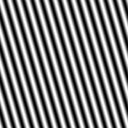
\includegraphics{img/03} 

\question[60] {\bf{Filtrando}}

En el mismo repositorio se encuentra la imágen con ruido \verb"clown.png".

Calcule la transformada de Fourier de la imágen, encuentre las frecuencias
que generan el patrón del ruido y elimínelas usando una máscara.
Reconstruya la imágen limpia.

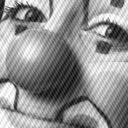
\includegraphics{img/clown}

\end{questions}

Imágenes tomadas de \url{http://www.imagemagick.org/Usage/fourier/}

Una presentación interesante sobre análisis de imágenes con Fourier:

\url{http://research.stowers-institute.org/efg/Report/FourierAnalysis.pdf}

Soundtrack: Morphine - \url{https://www.youtube.com/watch?v=eH2erx495io}

\end{document}
